\chapter{Introducción a grafos}

Un grafo es un objeto muy útil para modelar problemas. Es un conjunto de vértices conectados entre ellos por aristas. Normalmente los ilustramos así:

\begin{center}
	contenidos...
\end{center}


De forma que los círculos son los vértices y las líneas que unen los círculos son las aristas.

Los utilizamos para representar redes de objetos conectados o relacionados entre ellos. 

Por ejemplo, podemos usar un grafo para explicar quién conoce a quién. Supongamos que hay un grupo hay seis personas llamadas Alicia, Beto, Carla, Daniel, Elsa y Felipe. Si sabemos que las amistades son:
\begin{center}
	\begin{plimits}
		\item Alicia y Beto son amigos.
		\item Beto y Daniel son amigos.
		\item Alicia y Daniel son amigos.
		\item Carla y Felipe son amigos.
		\item Elsa no tiene amigos.
	\end{plimits}
\end{center}


Entonces podemos representar esto con un grafo, donde los vértices son las personas y las aristas muestran amistades:
\begin{center}
	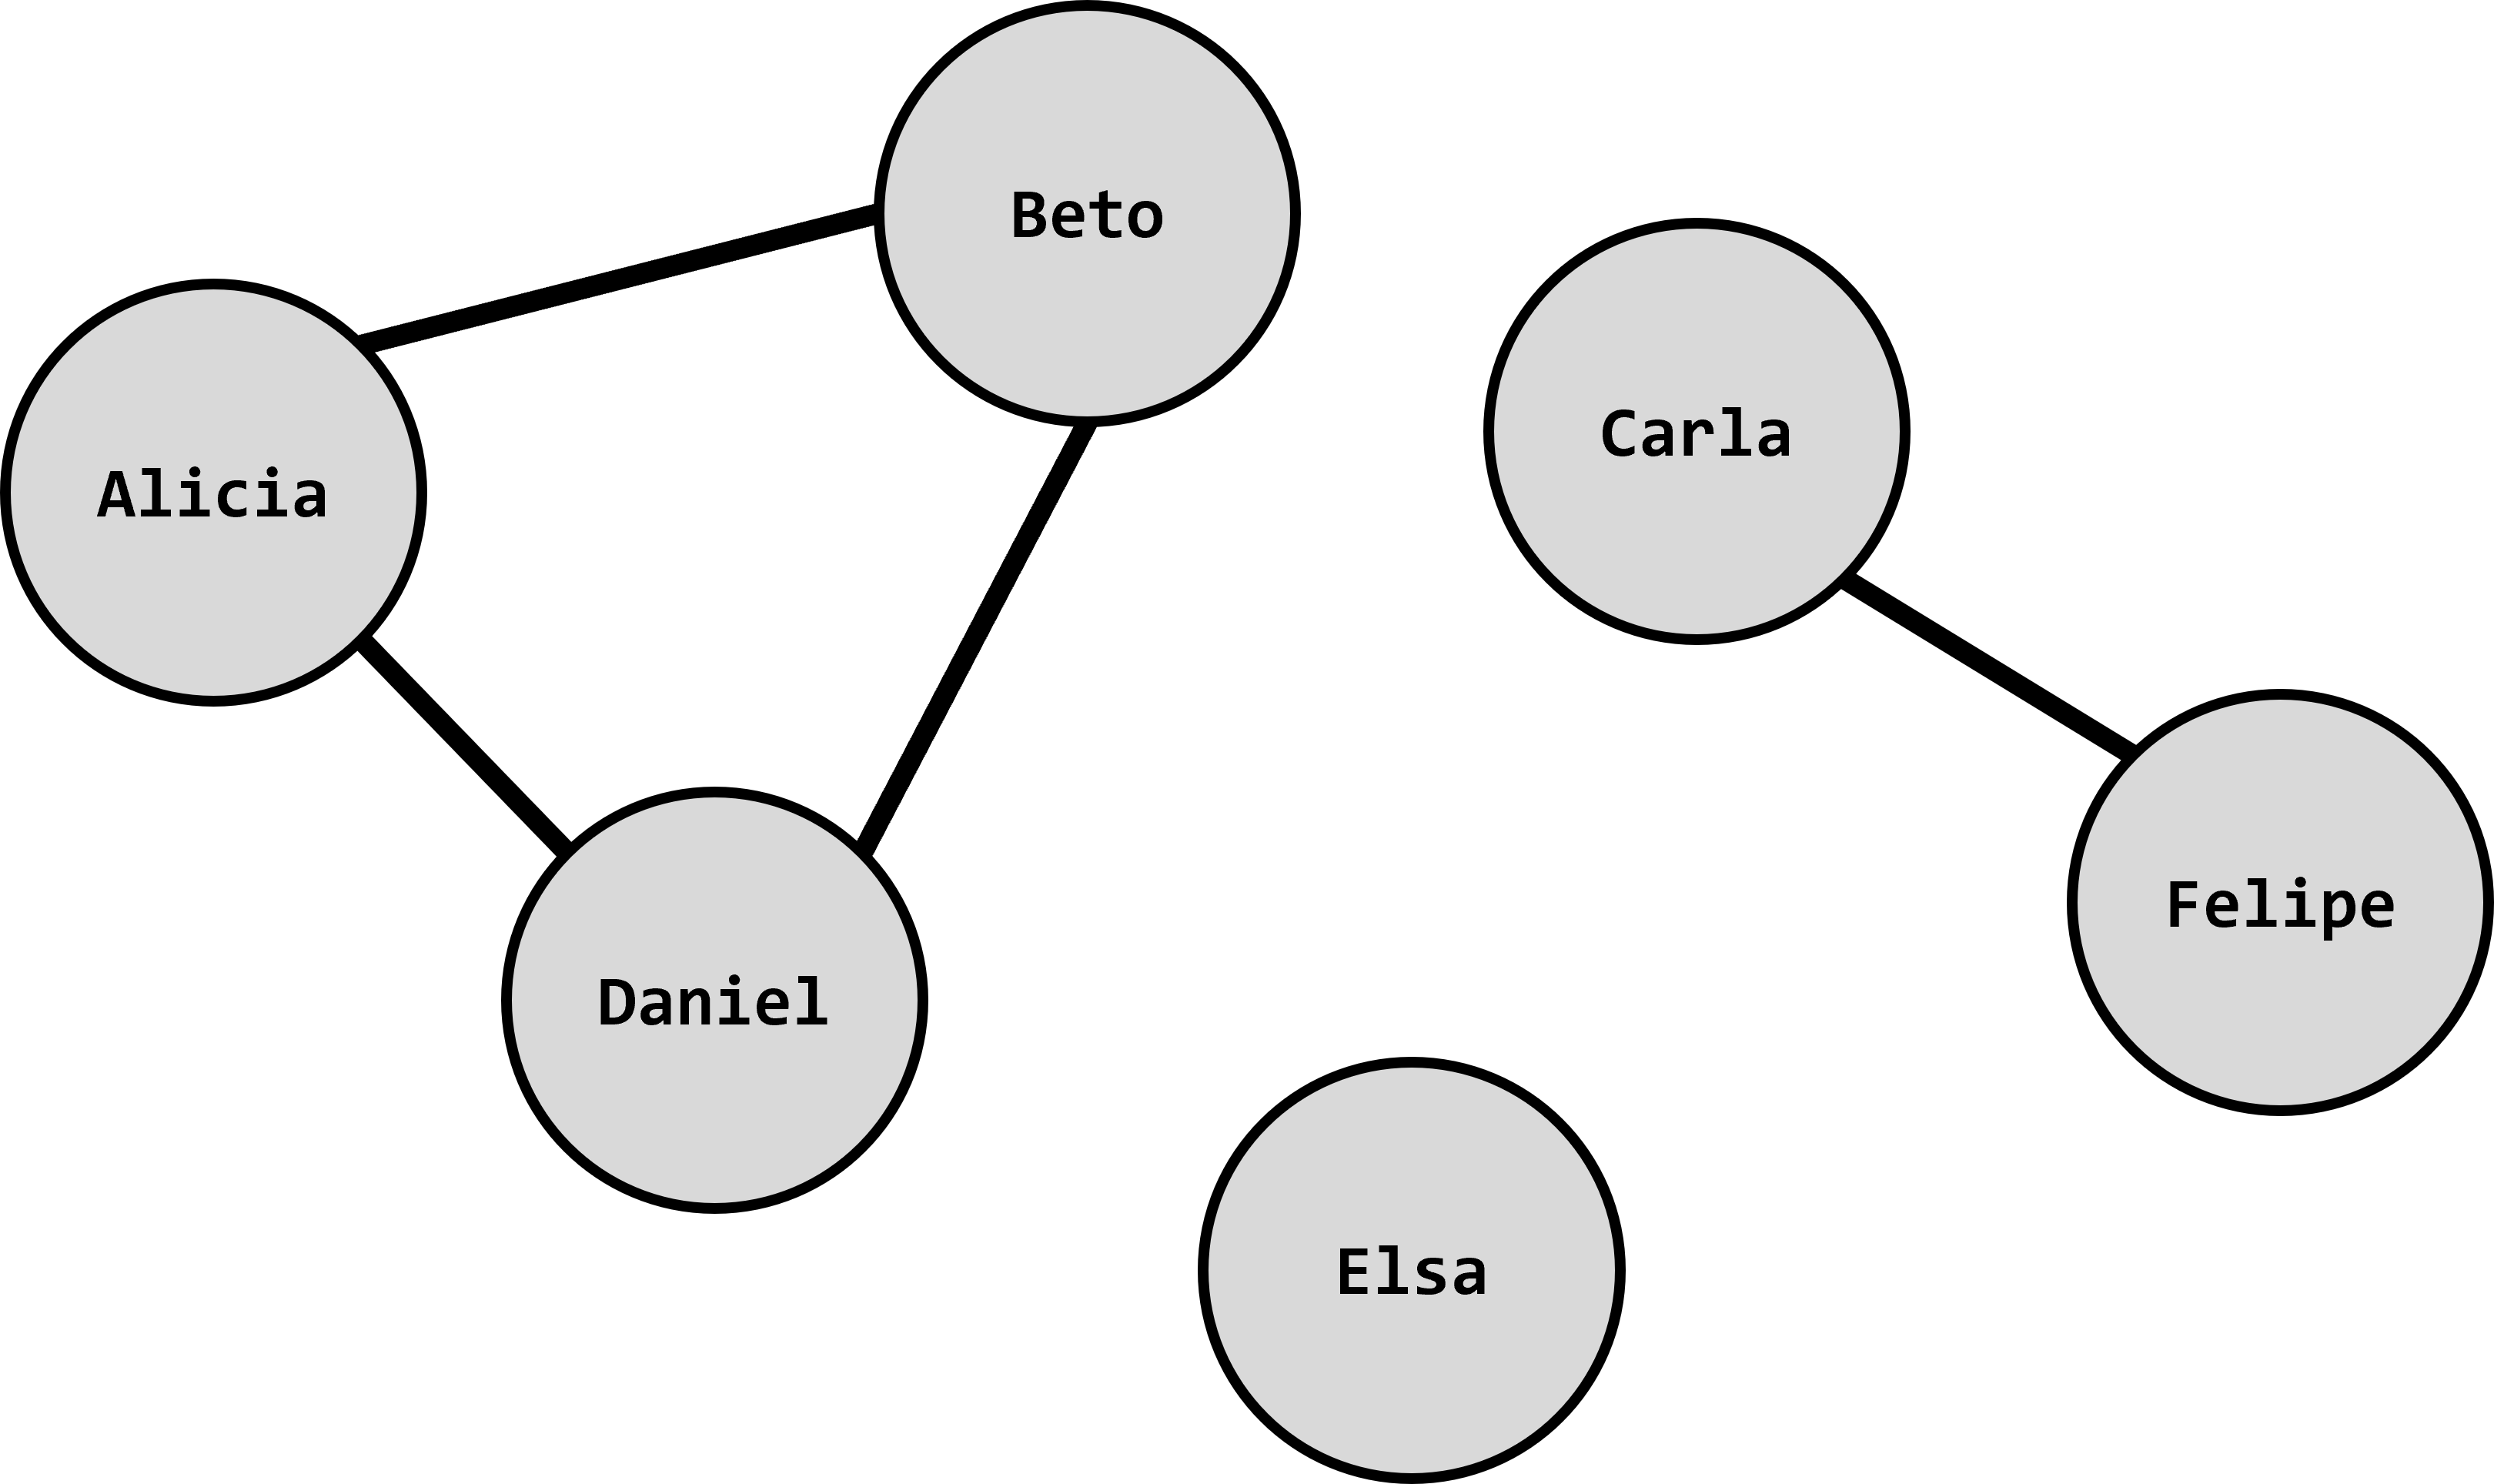
\includegraphics[scale=0.3]{grafos/amistades}
\end{center}

Entonces, los grafos son un conjunto de vértices y aristas. Mientras que las aristas son relaciones entre pares de vértices. Una arista siempre conecta exactamente dos vértices.

Ahora, el motivo por el cual es útil conocer grafos es que en los problemas de la olimpiada, muchas veces nos piden que resolvamos problemas en objetos con relaciones, ya sea un grupo de ciudades conectadas por carreteras, puertas del metro conectados con cables, números relacionados por cuales primos comparten, etc.

Conocer técnicas para trabajar con grafos se convierten por lo tanto en técnicas para todo problema que podamos imaginar como un grafo. 


\section*{Definiciones y notación}
A continuación escribiremos algunas definiciones de algunas palabras relacionadas.
\begin{itemize}
	\item \textbf{Nodo} Sinónimo de vértice.
	
	\item \textbf{Arco, conexión} Sinónimo de arista.
	
	\item \textbf{Vecino} Decimos que el vértice \(i\) es vecino de \(j\) si existe una arista de \(j\) que conecte con \(i\).
	
	\item \textbf{Grado} Decimos que el grado vértice \(i\) es la cantidad de aristas que se conectan con \(i\) y se suele escribir \(grado(i)\), en el ejemplo anterior el \(grado(Alicia)=2\) y \(grado(Elsa)=0\).
	
	\item \textbf{Adyacente} Se dice que el nodo \(i\) es adyacente a \(j\) si son vecinos.

	\item \textbf{G=(V,E)} Esta es la manera formal de definir un grafo.  Decimos que es una pareja, donde \(V\) es un conjunto de vértices y \(E\) un conjunto de aristas.
	
	\item \textbf{\{u, v\}} Representa una arista que conecta al vértice \(u\) con \(v\). 
\end{itemize}
